\documentclass[a4paper, fontsize=14pt]{article}
\usepackage{course_work}
\bibliography{course_work.bib}
\usepackage{graphs/gnuplot-lua-tikz}
%\setcounter{page}{4} %в зависимости от того, какой по счёту страницей должно быть оглавление!


\begin{document}
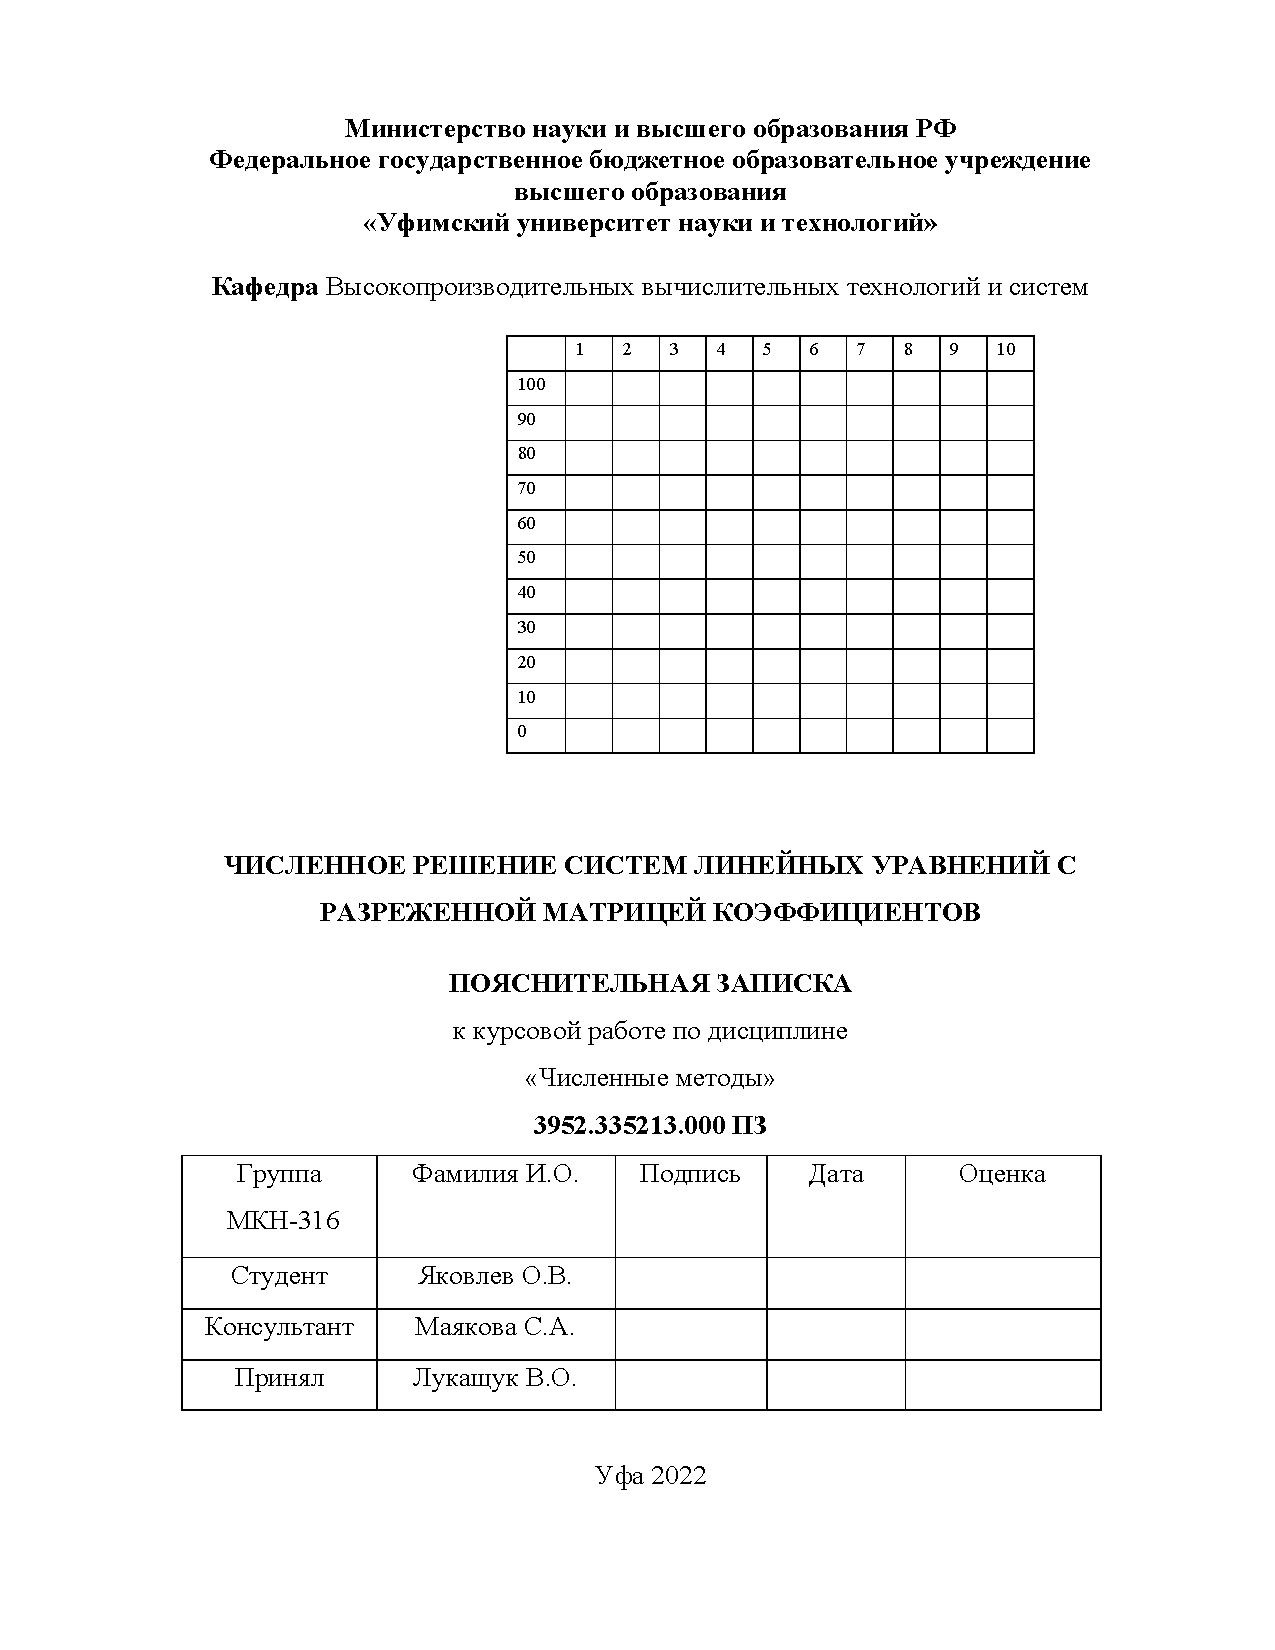
\includepdf[pages=-]{title-pages.pdf}
\newpage

\tableofcontents

\newpage

\section*{Введение}
\addcontentsline{toc}{section}{Введение}

Развитие вычислительной техники и вызванный этим процессом переход к более сложным (трехмерным, 
в произвольных геометрических областях) моделям в виде систем дифференциальных уравнений в 
частных производных и их дискретным аналогам на неструктурированных сетках, привел к 
необходимости решения больших разреженных систем линейных алгебраических уравнений с 
матрицами нерегулярной структуры.
% Написать про постановку задачи.

Целью данной курсовой работы является изучение способов решения СЛАУ с разреженной матрицей.
Для достижения данной цели были поставлены следующие задачи:
\begin{enumerate}
    \item Изучить литературу по теме "Численное решение систем линейных уравнений с разреженной
        матрицей коэффициентов"
    \item Разработать программу для решения СЛАУ с разреженной матрицей с помощью прямых и
        итерационных методов.
    \item Сравнить производительности программы при решении СЛАУ для каждого из методов.
\end{enumerate}
\newpage
\section{Хранение и обработка разреженных матриц}
Распространенным способом хранения несимметричных разряженных матриц произвольной структуры является
CSR. В нем разреженная матрица $A$ хранится с использованием следующих массивов:
\begin{itemize}
    \item \verb|value|, который содержит значения всех ненулевых элементов матрицы.
    \item \verb|cols|, который содержит номера столбцов, в которых стоит каждый ненулевой элемент.
    \item \verb|rows|, который содержит индекс начала строки в массивах \verb|values| и \verb|cols|.
\end{itemize}
Умножение матрицы, хранимой в таком формате, реализуется с помощью перебора элементов массива
\verb|values|, которые умножаются на элементы вектора $x$ с индексом из соответствующего
элемента массива \verb|cols|.\cite{bal} 

\section{Решение СЛАУ при помощи метода LU-разложения}

LU-разложение -- это представление матрицы $A$ в виде произведения двух матриц, $A=LU$, где
$L=(l_{ij})$ -- нижняя треугольная матрица, а $U=(u_{ij})$ -- верхняя треугольная матрица с
единичной диагональю. Элементы $l_{ij}$, $u_{i,j}$ определим из условия
$$\sum_{k=1}^{n}l_{ik}u_{kj} = a_{ij}\quad\forall i,j = 1,\dots,n$$
где матрицы $L$ и $U$ имеют вид 
$$L = 
\begin{pmatrix} 
    1 & 0 & \dots & 0 \\
    l_{21} & 1 & \dots & 0 \\
    \vdots & \vdots & \vdots &\vdots \\
    l_{n1} & l_{n2} & \dots & 1
\end{pmatrix}, 
U = 
\begin{pmatrix} 
    u_{11} & u_{12} & \dots & u_{1n} \\
    0 & u_{22} & \dots & u_{2n} \\
    \vdots & \vdots & \vdots &\vdots \\
    0 & 0 & \dots & u_{nn}
\end{pmatrix}
$$
Перемножив матрицы, получаем формулы для элементов матриц $L$ и $U$.
\begin{align*}
    l_{i1} &= a_{i1} \\
    u_{1i} &= \frac{a_{1j}}{l_{11}} \\
    l_{ij} &= a_{ij} - \sum_{k=1}^{j-1} l_{ik}u_{kj} \quad &i \ge j > 1\\
    u_{ij} &= \frac{1}{u_{ii}} \left(a_{ij} - \sum_{k=1}^{j-1} l_{ik}u_{kj}\right) \quad &1 < i < j\\
\end{align*}
Далее, СЛАУ можно представить в виде $LUx=b$. Решить систему можно разделив ее на две системы,
имеющие треугольные матрицы. 
$$
\begin{cases}
    Ly=b\\
    Ux=y
\end{cases}
$$
    Эти системы можно решить с помощью процедур прямого и обратного хода.\cite{kal}
\section{Метод бисопряженных градиентов}
    Системы векторов $\{x\}^m_{i=1}$ и $\{y\}^m_{i=1}$ называются
биортогональными, если скалярное произведение $(x_i , y_i)$ обращается в ноль при $i\neq j$.

    Пусть векторы $v_1$ и $w_1$ таковы, что $(v1 , w1) \neq 0$ и пусть системы векторов $\{y\}^m_{i=1}$
и $\{w\}^m_{i=1}$ определяются соотношениями:
\begin{align*}
    v_{i+1} &= A v_i - \alpha_i v_i - \beta_i v_{i-1} \quad &v_0 = 0\\
    w_{i+1} &= A^T w_i - \alpha_i w_i - \beta_i w_{i-1} \quad &w_0 = 0\\
    \alpha_i &= \frac{(Av_i,w_i)}{(v_i,w_i)} \\ 
    \beta_i &= \frac{(v_i,w_i)}{(v_{i-1},w_{i-1})} \quad &\beta_1 = 0
\end{align*}
тогда системы $\{y\}^m_{i=1}$ и $\{w\}^m_{i=1}$ биортогональны и каждая из них линейно независима и
образует базис в $K_m(v_1,A)$ и $K_m(w_1,A^T)$ соответственно.

Аналогично методу полной ортогонализации решение системы будет уточняться по формуле
$$ x_m = x_0 +\beta V_m T_m^{-1} e_1 $$
запишем LU-разложение для матрицы $T_m$
$$ T_m =  L_m U_m $$
Пусть $P_m = V_m U_m^{-1}$. Тогда $x_m$ имеет вид
$$ x_m = x_0 + \beta P_m L_m^{-1} e_1 $$
Аналогично определим $\bar{P}_m$
$$ \bar{P}_m = W_m (L_m^T)^{-1} $$
Тогда имеет место
$$ \bar{P}_m^T A P_m = I_m  D_m $$ 
где $D_m = (d_{ii}) = (v_i,w_i)$.

Таким образом, можно составить алгоритм \ref{alg:bicgm} решения СЛАУ с помощью метода бисопряженных
градиентов. \cite{saad}
\begin{algorithm}
    \caption{Метод бисопряженных градиентов}\label{alg:bicgm}
\begin{algorithmic}
    \State Выбрать начальное приближение $x_0$
    \State $r_0 \gets b - Ax_0$
    \State Выбрать вектор $\tilde{r}_0$, такой что $(r_0,\tilde{r_0}) \neq 0$
    \State $p_0 \gets r_0$
    \State $\tilde{p}_0 \gets \tilde{r}_0$
    \For{j=1,2,\dots}
        \State $\alpha_j \gets \frac{(r_j,\tilde{r}_j)}{(Ap_j,\tilde{p}_j)}$
        \State $x_{j+1} \gets x_{j} + \alpha_j p_j$
        \State $r_{j+1} \gets r_j - \alpha_j A p_j$
        \State $\tilde{r}_{j+1} \gets \tilde{r}_j - \alpha_j A^T \tilde{p}_j$
        \State $\beta_j \gets \frac{(r_{j+1},\tilde{r}_{j+1})}{(r_j,\tilde{r}_j)}$
        \State $ p_{j+1} \gets r_{j+1}+\beta_j p_j$
        \State $ \tilde{p}_{j+1} \gets \tilde{r}_{j+1}+\beta_j \tilde{p}_j$
    \EndFor

\end{algorithmic}
\end{algorithm}
    
    При решении СЛАУ с помощью итерационных методов, необходимо также знать достаточные условия
сходимости данных методов. Одним из таких условий может быть диагональное преобладание матрицы
системы.  
\section{Генерация симметричной матрицы с диагональным преобладанием}
Сперва для элементов матрицы, не лежащих на главной диагонали, генерируются случайные действительные
числа из интервала $[-1;1]$. Далее считается сумма модулей этих элементов. 
$$
    a_{ii} = \sum^{n}_{\substack{j=1\\ i \neq j}} |a_{ij}| 
$$
Значение этой суммы является значением элемента на главной диагонали данной строки матрицы. 

Далее необходимо сделать матрицу симметричной. Для этого элементам, расположенным ниже главной
диагонали присваиваем те же значения, что и у соответствующих элементов выше главной диагонали.
$$
    a_{ij} := a_{ji} \quad j<i
$$
\section{Результаты}
\subsection{Разработка структуры классов программной реализации}
В ходе выполнения курсовой работы была разработан класс \verb|compressed_matrix| для работы 
с разреженными матрицами. Класс реализует описанный ранее способ хранения разреженной матрицы CSR и
методы для работы с разреженными матрицами:
\begin{itemize}
    \item \verb|LU_decomposition| - LU-разложение матрицы 
    \item \verb|solve_L|
    \item \verb|solve_U|
    \item \verb|solve_BiCGStab|


\end{itemize}


\subsection{Анализ производительности программной реализации.}
\begin{figure}[h]
    \scriptsize
    \centering
    \include{graphs/comp.tex}
    \caption{Зависимость времени выполнения программы от размера матрицы.}
    \label{fig:comp}
\end{figure}
При решении СЛАУ малой размерности ($N \approx 10$), прямые могут оказаться быстрее.
Однако, при решении СЛАУ с матрицей больших размерностей, эффективны итерационные методы. 

На рисунке \ref{fig:comp} изображен график зависимости времени решения СЛАУ с разреженной матрицей
(матрица заполнена на 20\%, $\varepsilon = 10^{-5}$) при помощи прямого метода LU-разложения
матрицы системы и при помощи итерационного стабилизированного метода бисопряженных
градиентов(BiCGStab). График показывает, что скорость
сходимости итерационного метода сильно зависит от коэффициентов матрицы системы. Поэтому решение
систем с матрицей, обладающих сильным диагональным преобладанием происходит приблизительно в 2 раза
быстрее. Время решения СЛАУ с помощью метода LU-разложения не зависит от диагонального преобладания
матрицы системы. 

\begin{figure}[H]
    \scriptsize
    \centering
    \include{graphs/fill.tex}
    \caption{Зависимость времени выполнения программы от заполненности матрицы.}
    \label{fig:fill}
\end{figure}
Также время решения системы может зависеть от разреженности матрицы. На рисунке \ref{fig:fill}
изображен график зависимости времени решения СЛАУ($N=800$, $\varepsilon = 10^{-5}$) методами LU-разложения и BiCGStab от заполненности
матрицы(отношения количества ненулевых коэффициентов матрицы к общему их количеству). На графике
видно, что при увеличении заполненности время решения СЛАУ с помощью итерационного метода тоже
увеличивается. Поэтому для систем небольшой размерности с плотно заполненной матрицей можно
применять прямые методы решения СЛАУ.

\newpage

\section*{Заключение}
\addcontentsline{toc}{section}{Заключение}
% Выводы из анализа тоже добавить сюда
В ходе выполнения курсовой работы была изучена литература по теме <<Численное решение систем
линейных уравнений с разреженной матрицей коэффициентов>>. 
Далее была разработана программа для решения СЛАУ с разреженной матрицей с помощью прямых и
итерационных методов.  Наконец было произведено сравнение производительности программы при
решении СЛАУ для каждого из методов. Таким образом были изучены способы решения СЛАУ с разреженной
матрицей.


\newpage

\addcontentsline{toc}{section}{Список литературы}

\printbibliography

\end{document}
